\documentclass[dvipdfmx]{jsarticle}
\usepackage{graphicx}

\begin{document}

\title{強度計算書}
\author{河村勇人}

\maketitle

\begin{tabular}{ll}
 品名 & JBA Upper Control Arms for 2002-2007 lifted Jeep Liberty's \\
 メーカー & JBA Offroad\footnotemark[1] \\
 適応車種 & Jeep チェロキー (英語名 Jeep Liberty) \\
 適応型式 & GH-KJ37
\end{tabular}\linebreak
\footnotetext[1]{https://jbaoffroad.com}

JBA Upper Control Arms for 2002-2007 lifted Jeep Liberty's (以下、アッパーアーム)はJeepチェロキー(型式GH-KJ37)での使用を目的に専用設計され、高い耐久性を含む純正のアッパーアームを超えるパフォーマンスを獲得する目的で設計された部品であるが、製造者がアメリカ合衆国を拠点としており日本国の車検制度を想定していないことから、メーカーから強度計算書に相当する資料が提供されていない。
一方で、アッパーアームの材質と寸法についてはメーカーより情報提供を受けたため、材料力学における一般的な強度計算式を用いて当該部品がJeepチェロキーでの使用に耐えることを証明する。

\section{基礎データ}

車軸重計算の対象となる車両のデータを以下に示す。

\newcommand{\Wf}{1030}
\newcommand{\Wb}{2650}
\newcommand{\Sone}{1300}
\newcommand{\None}{2}
\newcommand{\Stwo}{2100}
\newcommand{\Ntwo}{3}

\begin{tabular}{lll}
 前軸荷重(Wf) & \Wf kg & 車検証記載 \\
 ホイールベース(L) & \Wb mm & 実測 \\
 前軸からの1列目シート距離(S1) & \Sone mm & 実測 \\
 1列目シート定員(N1) & \None & \\
 前軸からの2列目シート距離(S2) & \Stwo mm & 実測 \\
 2列目シート定員(N2) & \Ntwo &
\end{tabular}\linebreak

強度計算の対象となるアッパーアームのデータを以下に示す。

\newcommand{\AOD}{26.92}
\newcommand{\AID}{19.05}
\newcommand{\YSTMPA}{448}
\newcommand{\TSTMPA}{517}

\begin{tabular}{lll}
 材質 & 1026 ASTM A513 Type 5 DOMチューブ & メーカー提供情報 \\
 重量 & 14lbs (6.35Kg) & メーカー提供情報 \\
 チューブ外径(OD) & \AOD mm & メーカー提供情報 \\
 チューブ内径(ID) & \AID mm & メーカー提供情報 \\
 1026 ASTM A513-5 DOM 降伏強度 & \YSTMPA Mpa & 鋼材メーカー公開情報\footnotemark[2] \\
 1026 ASTM A513-5 DOM 引張強度 & \TSTMPA Mpa & 鋼材メーカー公開情報\footnotemark[2]
\end{tabular}
\footnotetext[2]{https://www.boyersteel.com/resource-astm-specifications/a513-t-5-d-o-m/}

\section{アッパーアーム強度の検討}

Jeepチェロキーにおけるフロントアッパーアームに掛かる荷重を以下の通り計算する。
定員1名あたりの重量を一般的な荷重計算で用いられる55Kgとした場合、車両総前軸重は以下の通り求められる。

\begin{displaymath}
  車両総前軸重 = Wf + 55 * \{N1(L-S1)+N2(L-S2)\} / L = 1120.28Kg
\end{displaymath}

したがって総片軸重は以下となる。さらに乗用車稼働部に適用される一般的負荷係数2.5を乗じて片前軸最大荷重とする。

\begin{displaymath}
  車両総片前軸重 = 車両総前軸重 / 2 = 560.14Kg
\end{displaymath}
\begin{displaymath}
  片前軸最大荷重 = 車両総片前軸重 * 2.5 = 1400.35Kg
\end{displaymath}


続いてアッパーアームの強度を以下の通り計算する。
基礎データで示した通り、メーカー提供情報としてアッパーアームは標準規格化された1026 ASTM A513 Type 5 DOMチューブ(以下1026DOM)材によって製造されている。
1026DOMの強度については複数のメーカーより公開情報として提供されており\footnotemark[2]、単位面積あたりの降伏強度は\YSTMPA Mpa, 引張強度は\TSTMPA Mpaである。1Mpa = 0.10197Kgf/mm2であるから、単位変換すると以下となる。

\begin{displaymath}
  降伏強度(Kgf/mm2) = 降伏強度(Mpa) * 0.10197 = 45.68Kgf/mm^2
\end{displaymath}
\begin{displaymath}
  引張強度(Kgf/mm2) = 引張強度(Mpa) * 0.10197 = 52.72Kgf/mm^2
\end{displaymath}

アッパーアームで採用されているチューブの外径/内径については基礎データで示した通りであり、そこからチューブの最小断面積は以下の通り求められる。

\begin{displaymath}
  最小断面積(d1) = \{(OD / 2.0) ^ 2 - (ID / 2.0) ^ 2\} * 3.14 = 284.0mm^2
\end{displaymath}

今回検討するのはせん断力であるため、基礎データで示した1026DOMの引張強度に対して一般的に用いられる変換式である$\sqrt{3}$で割ることでせん断強さを求め、上記の断面積と合わせて1026DOMチューブのせん断力を以下の通り計算する。

\begin{displaymath}
  降伏せん断強さ = 降伏強度(Kgf/mm2) / \sqrt{3} = 26.37Kgf/mm^2
\end{displaymath}
\begin{displaymath}
  破壊せん断強さ = 引張強度(Kgf/mm2) / \sqrt{3} = 30.44Kgf/mm^2
\end{displaymath}
\begin{displaymath}
  降伏せん断力 = d1 * 降伏せん断強さ = 7489.08Kg
\end{displaymath}
\begin{displaymath}
  破壊せん断力 = d1 * 破壊せん断強さ = 8644.96Kg
\end{displaymath}

上記の通り示されたせん断力を、前軸最大荷重で割ると以下のようになる。尚、本来前軸荷重はアッパーアーム、ロアアーム、スプリングといった部品に分散して荷重されるものであるため、実際にアッパーアームに荷重される割合は上に示した計算結果の1/3程度になると考えられるが、ここでは仮に片前軸最大荷重の100\%がアッパーアーム単体に荷重された場合でも十分に耐えることを示すため、片前軸最大荷重をそのまま用いて計算する。
図\ref{fig:arm}に示された外観図の通り、アッパーアームは2本の1026DOMチューブによって構成される部品であるため、1026DOMチューブ1本あたりに荷重されるのは片前軸最大荷重の半分となることから以下のように計算できる。

\begin{displaymath}
  降伏安全率 = 降伏せん断力 / \frac{片前軸最大荷重}{2} = 10.7
\end{displaymath}
\begin{displaymath}
  破壊安全率 = 破壊せん断力 / \frac{片前軸最大荷重}{2} = 12.35
\end{displaymath}

上記の通り計算された安全率は、乗用車に関して一般に期待される降伏安全率1.3に対して約8.2倍、破壊安全率1.6に対して約7.7倍であり、以上のことから当該アッパーアームはJeepチェロキーにおける使用に対して十分な強度を持つ。

\begin{figure}[h]
  \centering
  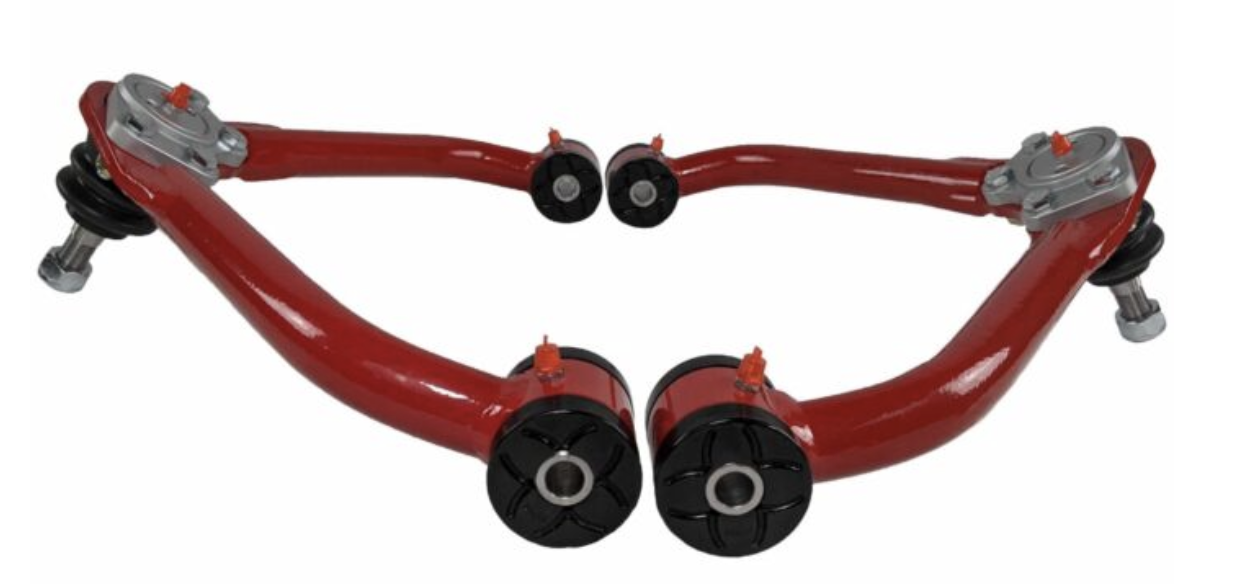
\includegraphics[scale=0.5]{arm-pic.png}
  \caption{JBA Upper Control Arms for 2002-2007 lifted Jeep Liberty's}
  \label{fig:arm}
\end{figure}

\begin{figure}
\centering
\begin{minipage}{.5\textwidth}
  \centering
  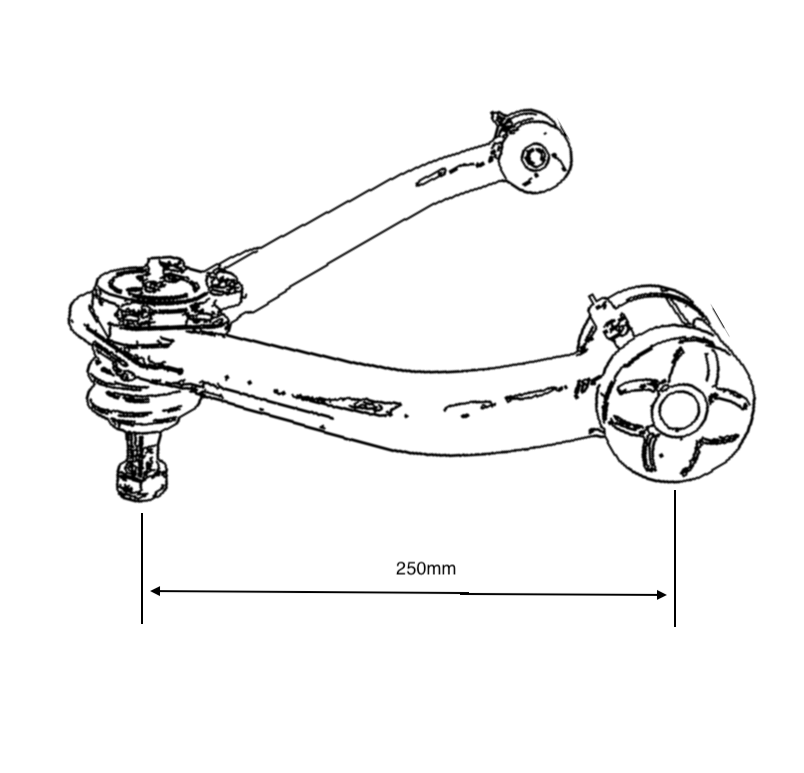
\includegraphics[scale=.3]{arm-detail-1.png}
\end{minipage}%
\begin{minipage}{.5\textwidth}
  \centering
  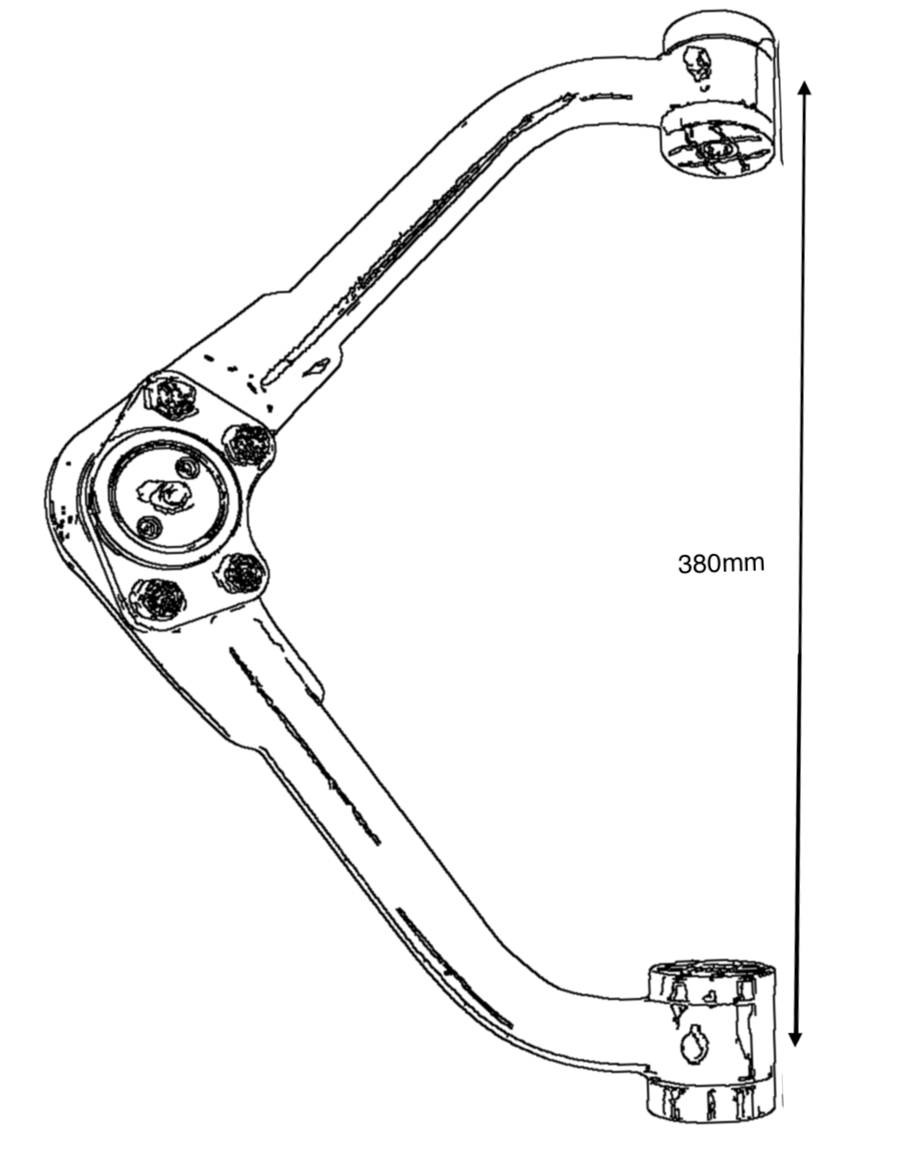
\includegraphics[scale=.2]{arm-detail-2.png}
\end{minipage}
\caption{アッパーアーム詳細寸法}
\label{fig:arm-detail}
\end{figure}

\end{document}
